\chapter{Metodología y Análisis del Sistema Propuesto:}\label{chapter:proposal}

¿Cómo se va a construir el sistema y por qué se eligió esta forma?


\section{Metodologías de desarrollo de software}
\label{section:metodologias_desarrollo}

Una metodología de desarrollo de software es un marco de trabajo estructurado que organiza, planifica y controla el proceso de construcción de un sistema. Su relevancia radica en que permite reducir la complejidad del desarrollo al dividir el proyecto en etapas gestionables, establecer un lenguaje común entre los involucrados y mejorar la calidad del producto final mediante prácticas sistemáticas de ingeniería de software \cite{Pfleeger2015}.

En este contexto, existen diversas metodologías de desarrollo, cada una con enfoques particulares para la gestión del ciclo de vida del software.

\begin{itemize}

\item El modelo en cascada se basa en un enfoque secuencial y lineal del desarrollo, donde las fases de análisis, diseño, implementación, pruebas y mantenimiento se ejecutan de manera ordenada y progresiva. Cada fase debe completarse antes de iniciar la siguiente, lo que proporciona un alto nivel de control y documentación, aunque limita la flexibilidad ante cambios durante el desarrollo \cite{Sommerville2015, Royce1987}.

\item Scrum es un marco de trabajo ágil basado en el desarrollo iterativo e incremental, en el cual el sistema se construye mediante ciclos cortos llamados \textit{sprints}. Cada iteración produce un incremento funcional del sistema, permitiendo la adaptación continua a cambios y la inspección constante del progreso \cite{Schwaber2020}.

\item Kanban es un método de gestión del flujo de trabajo orientado a la mejora continua del proceso de desarrollo. Se basa en la visualización del trabajo, la limitación del trabajo en curso y la optimización del flujo de tareas, permitiendo una entrega continua sin necesidad de iteraciones fijas \cite{Anderson2010}.

\item Extreme Programming (XP) es una metodología ágil centrada en la calidad técnica del software. Se fundamenta en valores como la simplicidad, la comunicación y la retroalimentación constante, e incorpora prácticas como el desarrollo guiado por pruebas, la refactorización continua y la programación en parejas, con el objetivo de mejorar la mantenibilidad y robustez del sistema \cite{Beck2004}.

\end{itemize}


\subsection{Comparación de metodologías de desarrollo aplicadas al sistema}
\label{subsection:comparacion_metodologias_sistema}

Con el objetivo de seleccionar la metodología más adecuada para el desarrollo del sistema de gestión y autorreporte de ESAVI , se realizó un análisis comparativo entre los diferentes enfoques de desarrollo de software, evaluando su comportamiento en relación con las características específicas del proyecto.

Entre los criterios considerados se incluyen la variabilidad de los requisitos, la necesidad de desarrollo incremental, la mantenibilidad del código, la compatibilidad con una arquitectura desacoplada, la capacidad de adaptación a cambios en el diseño y la resiliencia ante interrupciones operativas durante el desarrollo, tales como cortes de energía eléctrica y problemas de conectividad.


\begin{table}[h!]
\centering
\renewcommand{\arraystretch}{1.3}
\begin{tabular}{|p{3.5cm}|p{2.8cm}|p{2.8cm}|p{2.8cm}|p{2.8cm}|}
\hline
\textbf{Criterio} & \textbf{Cascada} & \textbf{Scrum} & \textbf{Kanban} & \textbf{XP} \\
\hline

Flexibilidad ante cambios de requisitos y rediseño 
& Baja. Enfoque secuencial con poca capacidad de adaptación una vez avanzadas las fases. 
& Alta. Permite adaptación iterativa de requisitos y ajustes entre entregas. 
& Alta. Facilita la reorganización continua de tareas y prioridades. 
& Alta. Soporta cambios mediante refactorización continua y desarrollo incremental. \\
\hline

Calidad y mantenibilidad del código 
& Baja. No incorpora prácticas técnicas específicas de calidad. 
& Media. Depende de las prácticas del equipo de desarrollo. 
& Baja. No influye directamente en la calidad del código. 
& Alta. Promueve refactorización, simplicidad y buenas prácticas de desarrollo. \\
\hline

Soporte para arquitectura modular (Clean Architecture) 
& Baja. Diseño rígido definido al inicio con poca adaptabilidad. 
& Alta. Permite evolución progresiva de la arquitectura. 
& Media. No define estructura arquitectónica. 
& Alta. Favorece la separación de responsabilidades y modularidad del sistema. \\
\hline

Adecuación al contexto de desarrollo individual y restricciones operativas 
& Baja. Requiere planificación rígida y secuencial. 
& Media. Diseñado para equipos, requiere adaptación en contexto individual. 
& Alta. Flexible y adecuado para gestión individual de tareas. 
& Alta. Compatible con desarrollo individual y mejora continua del código. \\
\hline

\end{tabular}
\caption{Comparación de metodologías de desarrollo según criterios del sistema}
\label{tab:comparacion_metodologias_4criterios}
\end{table}

\subsection{Aplicación Práctica de Scrum en el Proyecto}

Para el desarrollo del sistema de autorreporte de ESAVI se seleccionó Scrum por su flexibilidad para gestionar entregas incrementales y adaptarse a cambios en los requisitos, decisión respaldada por la experiencia previa del autor, las tutoras y el equipo revisor del Instituto Finlay de Vacunas en metodologías ágiles. Dado el carácter unipersonal del proyecto, el desarrollador asumió los roles de \textit{Scrum Master} y Equipo de Desarrollo, mientras que las tutoras oficiaron como \textit{Product Owner}, definiendo requisitos y validando entregas sin intervenir en aspectos técnicos \cite{Schwaber2020}.


El trabajo se estructuró en \textbf{cuatro \textit{Sprints}} de dos semanas. Antes de cada uno, se realizaba una \textit{Sprint Planning} donde las tutoras comunicaban las prioridades y se acordaban el objetivo y las tareas del ciclo. Durante la iteración, el progreso se controlaba mediante un tablero Kanban. Las funcionalidades desarrolladas fueron:
\begin{itemize}
    \item \textbf{\textit{Sprint} 1:} Arquitectura base y formulario de autorreporte con datos del paciente, vacuna administrada y tipo de evento adverso.
    \item \textbf{\textit{Sprint} 2:} Anonimización de datos y almacenamiento seguro de reportes.
    \item \textbf{\textit{Sprint} 3:} Panel de seguimiento de casos notificados para profesionales de salud.
    \item \textbf{\textit{Sprint} 4:} Refinamiento de interfaz, validaciones clínicas y preparación para despliegue.
\end{itemize}
Al cierre de cada \textit{Sprint}, se efectuaba una \textit{Sprint Review} con las tutoras para verificar el cumplimiento de requisitos y plazos, y una \textit{Sprint Retrospective} individual para ajustar el proceso. Esta dinámica permitió incorporar, desde el segundo ciclo, nuevos criterios de clasificación de eventos adversos de la OMS sin afectar la fecha de entrega \cite{Schwaber2020}.

\section{Levantamiento y análisis de requisitos}
\label{section:requisitos}

En esta sección se presentan los requisitos del sistema, obtenidos a partir del análisis del flujo de farmacovigilancia del Instituto Finlay de Vacunas. Se clasifican en requisitos funcionales —las acciones que el sistema debe realizar— y no funcionales —los atributos de calidad bajo los cuales debe operar—.

\subsection{Requisitos funcionales}
\label{subsection:requisitos_funcionales}

El sistema web de autorreporte de \gls{esavi} se centra en la captura, gestión y seguimiento de reportes, así como en el soporte al análisis de la información por parte del personal autorizado. A continuación, se describen los principales requerimientos funcionales:

\begin{itemize}

\item \textbf{RF-01. Registro de eventos adversos:}  
El sistema deberá permitir a los usuarios registrar reportes de eventos adversos post-vacunación mediante un formulario web estructurado.

\item \textbf{RF-02. Gestión de información del reporte:}  
El sistema deberá permitir la captura de datos del paciente, vacunas administradas, y descripción del evento adverso, incluyendo la posibilidad de registrar múltiples eventos en un mismo reporte.

\item \textbf{RF-03. Identificación del reporte:}  
El sistema deberá generar automáticamente un código único de notificación o identificación para cada reporte registrado exitosamente.

\item \textbf{RF-04. Validación de formularios:}  
El sistema deberá validar los campos obligatorios del formulario antes de permitir el envío del reporte.

\item \textbf{RF-05. Almacenamiento de reportes:}  
El sistema deberá almacenar los reportes en una base de datos centralizada para su posterior análisis y seguimiento.

\item \textbf{RF-06. Gestión del estado del reporte:}  
El sistema deberá permitir la actualización del estado de los reportes dentro del flujo de farmacovigilancia (por ejemplo: pendiente, en revisión, validado, cerrado).

\item \textbf{RF-07. Consulta y filtrado de reportes:}  
El sistema deberá permitir la búsqueda y filtrado de reportes según criterios como fecha, vacuna, severidad y datos demográficos.

\item \textbf{RF-08. Visualización de información:}  
El sistema deberá permitir la visualización detallada de cada reporte de evento adverso.

\item \textbf{RF-09. Gestión de usuarios:}  
El sistema deberá permitir la autenticación de usuarios y la administración de roles para el acceso a funcionalidades específicas.

\item \textbf{RF-10. Generación de estadísticas:}  
El sistema deberá generar reportes estadísticos y visualizaciones gráficas para el análisis de los eventos adversos registrados.

\item \textbf{RF-11. Exportación de datos:}  
El sistema deberá permitir la exportación de información en formatos utilizados para análisis o reporte institucional.

\item \textbf{RF-12. Notificaciones del sistema:}  
El sistema deberá generar notificaciones automáticas basadas en eventos del flujo de gestión de reportes de eventos adversos, dirigidas a los usuarios según su rol dentro del sistema.

\end{itemize}

\subsection{Requerimientos no funcionales del sistema}
\label{subsection:requerimiento_no_funcionales}

El sistema web de autorreporte de eventos adversos post-vacunación deberá cumplir con un conjunto de requerimientos no funcionales orientados a garantizar la calidad, seguridad, disponibilidad y usabilidad de la plataforma.

\begin{itemize}

\item \textbf{RNF-01 Eficiencia y usabilidad del registro.}  
El sistema deberá cumplir con los siguientes criterios en el proceso de reporte de un evento adverso:
\begin{itemize}
    \item Completarse en un tiempo promedio menor a 2 minutos por parte de un usuario familiarizado con la plataforma.
    \item Presentar una interfaz intuitiva\footnote{Se entiende por interfaz intuitiva aquella que puede ser utilizada sin entrenamiento previo, siguiendo patrones de diseño web convencionales reconocidos por el usuario promedio.} y fácil de usar para usuarios con diferentes niveles de alfabetización digital.
    \item Basar la captura de datos principalmente en elementos estructurados como listas desplegables, botones de selección y casillas de verificación, minimizando el uso de texto libre.
\end{itemize}

\item \textbf{RNF-02. Accesibilidad:}  
El sistema deberá cumplir con las pautas de accesibilidad WCAG 2.1\footnote{Web Content Accessibility Guidelines (WCAG) 2.1: estándar internacional que establece criterios para hacer el contenido web accesible a personas con discapacidad visual, auditiva, motriz y cognitiva. El nivel AA es el umbral recomendado para sitios web gubernamentales y de salud.} nivel AA, garantizando su uso por personas con diferentes capacidades físicas y sensoriales.

\item \textbf{RNF-03. Diseño responsivo:}  
El sistema deberá adaptarse adecuadamente a diferentes dispositivos y resoluciones de pantalla, incluyendo computadoras de escritorio, tabletas y dispositivos móviles.

\item \textbf{RNF-04 Rendimiento.}  
El sistema deberá cargar sus páginas en un tiempo inferior a 3 segundos y procesar el envío de un reporte en menos de 5 segundos bajo condiciones normales de conectividad.

\item \textbf{RNF-05. Seguridad de la información:}  
El sistema deberá garantizar la confidencialidad, integridad y disponibilidad de los datos mediante mecanismos de autenticación, control de acceso y cifrado de información sensible.

\item \textbf{RNF-06. Auditoría y trazabilidad:}  
El sistema deberá registrar las acciones relevantes realizadas por los usuarios, incluyendo creación, modificación y actualización de reportes, con fines de auditoría y control institucional.

\item \textbf{RNF-07 Mantenibilidad.}  
El sistema deberá estar diseñado de manera modular, con separación clara entre sus componentes, facilitando la corrección de errores, la incorporación de nuevas funcionalidades y la escalabilidad del sistema.

\item \textbf{RNF-08. Compatibilidad:}  
El sistema deberá ser compatible con los principales navegadores web modernos: Google Chrome, Mozilla Firefox, Microsoft Edge y Safari.

\end{itemize}

\subsection{Reglas de negocio}
\label{subsection:reglas_negocio}

A continuación se describen las reglas que rigen la lógica de los formularios y el procesamiento de reportes dentro del sistema:

\begin{itemize}

\item \textbf{RN-01 Unicidad de vacuna por fecha.} No se puede registrar la misma vacuna más de una vez en la misma fecha para un mismo sujeto vacunado.

\item \textbf{RN-02 Vacunación previa al evento.} La fecha del primer evento adverso reportado debe ser siempre posterior a la fecha de la vacunación más reciente registrada en el reporte.

\item \textbf{RN-03 Eventos posteriores al fallecimiento.} Si en alguno de los eventos adversos se declara como desenlace el fallecimiento del sujeto vacunado, no se permitirá registrar nuevos eventos adversos con fecha posterior a la fecha de muerte.

\end{itemize}

\section{Modelado del sistema}

\subsection{Diagrama de casos de uso}

En esta sección se exponen las acciones que pueden realizar los distintos tipos de usuarios dentro de la plataforma, detalladas a través de un diagrama de casos de uso\footnote{Diagrama de casos de uso: Forma de diagrama de comportamiento UML mejorado. Sirve para especificar la comunicación y el comportamiento de un sistema mediante su interacción con los usuarios y/u otros sistemas.}. 
Para una mejor comprensión, se han categorizado las funcionalidades según el rol del actor y las dependencias lógicas de inclusión y extensión que rigen el sistema.

\subsubsection{Identificación de Actores}

De acuerdo con el modelado funcional, se han identificado cinco actores principales que interactúan con el sistema de gestión de vacunación y \gls{esavi}:

\begin{itemize}
    \item \textbf{Usuario:} Actor abstracto que representa la base de permisos comunes. De él heredan todos los roles que requieren autenticación en el sistema.
    \item \textbf{Jefe de Vacunación Municipal:} Hereda de Usuario. Responsable de la supervisión local, encargado de la gestión del personal médico y la distribución de la carga de trabajo.
    \item \textbf{Médico Evaluador:} Hereda de Usuario. Profesional sanitario encargado del análisis clínico de los eventos reportados.
    \item \textbf{Administrador:} Hereda de Usuario. Perfil técnico responsable del mantenimiento de los parámetros del sistema (catálogos) y la gestión de usuarios de alto nivel.
    \item \textbf{Reportante:} Actor independiente sin autenticación. Encargado de la entrada inicial de datos y el seguimiento de los reportes generados mediante el número de notificación.
\end{itemize}

\subsubsection{Análisis de los Casos de Uso}
A continuación, se describen las funcionalidades principales representadas en la Figura \ref{fig:diagrama_casos_uso}, detallando la lógica de negocio asociada a cada interacción:

\begin{figure}[H]
    \centering
    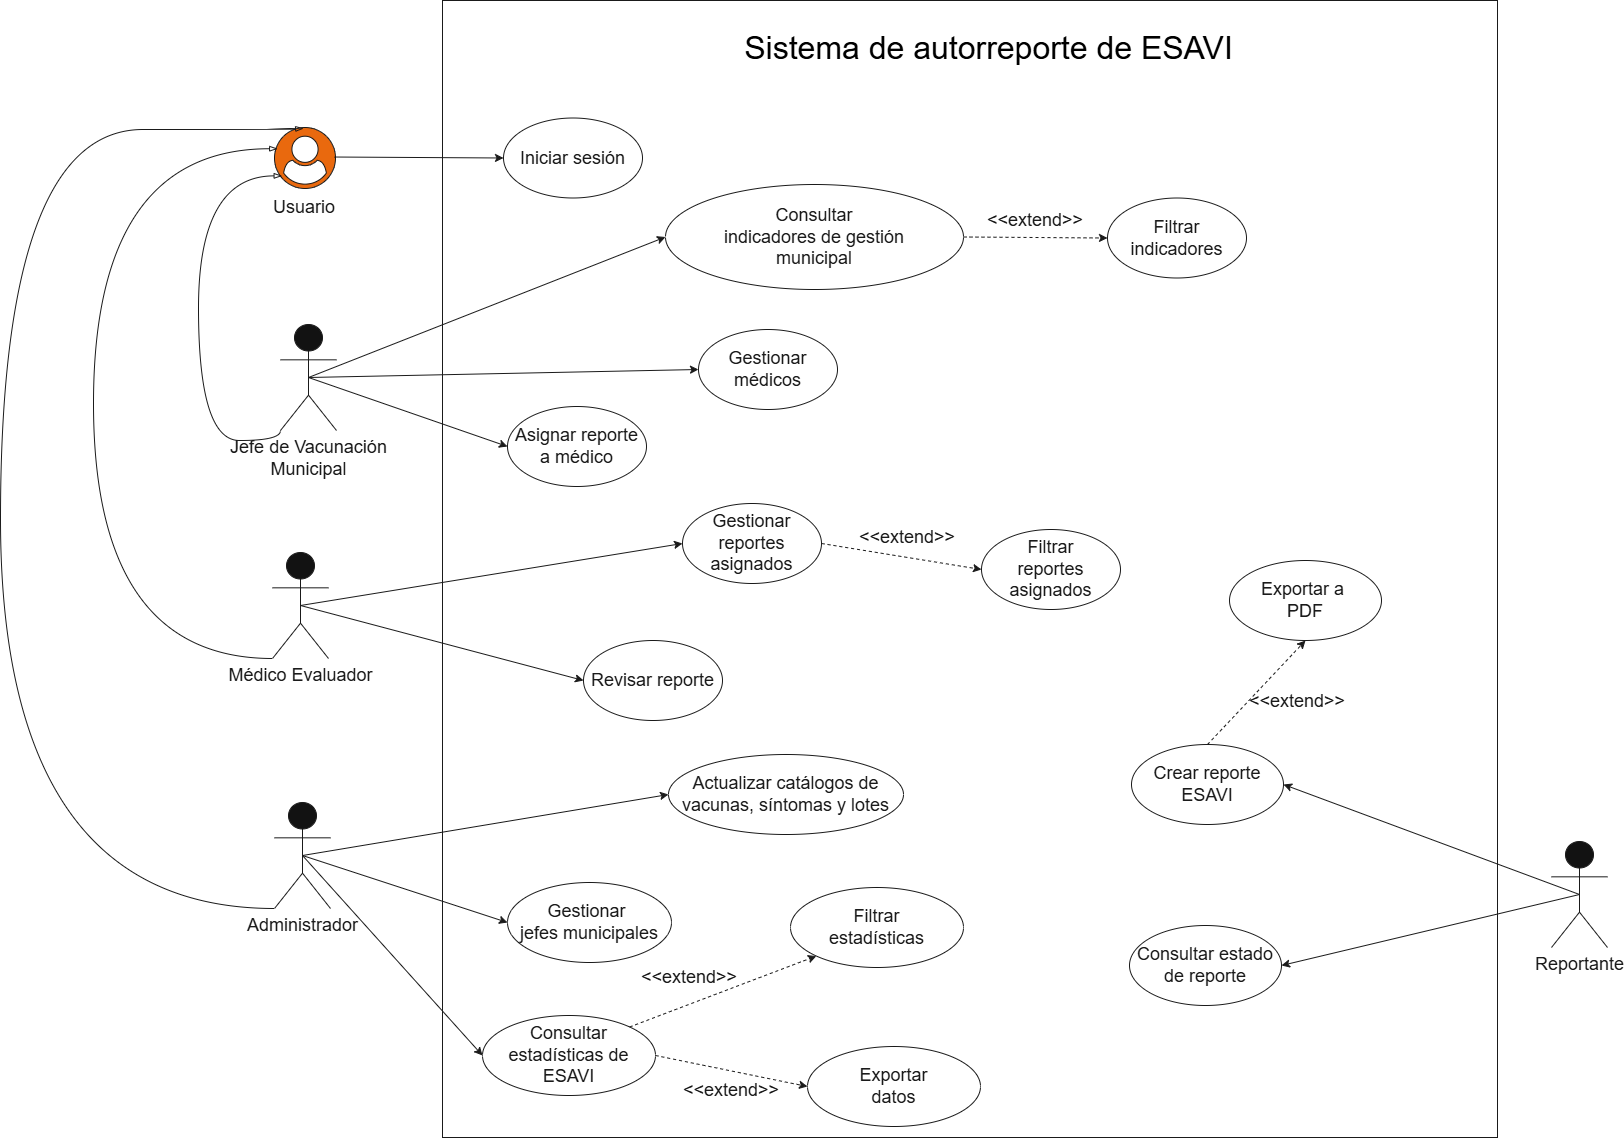
\includegraphics[scale=0.2]{Graphics/Cap3/diagrama_casos_uso_white.drawio (4).png}
    \caption[Diagrama de casos de uso]{Diagrama de casos de usos. Fuente: elaboración propia.}
    \label{fig:diagrama_casos_uso}
\end{figure}


\begin{itemize} 
    \item \textbf{Iniciar sesión:} Caso de uso base que permite el acceso controlado a la plataforma según las credenciales del usuario.
    \item \textbf{Gestión de reportes (Reportante):}
        \begin{itemize}
            \item \textbf{Crear reporte ESAVI:} Permite el ingreso de un nuevo evento adverso. Este caso de uso posee una relación de tipo \textit{extend} hacia \textbf{Exportar a PDF}, lo que indica que el usuario puede, opcionalmente, generar un comprobante documental tras completar el registro.
            \item \textbf{Consultar estado de reporte:} Permite al reportante verificar el estado de sus envíos previos ingresando el número de notificación.
        \end{itemize}

    \item \textbf{Gestión Clínica (Médico Evaluador):}
    \begin{itemize}
        \item \textbf{Gestionar reportes asignados:} Vista principal del médico donde visualiza su carga laboral. De manera opcional (\textit{extend}), puede aplicar \textbf{Filtrar reportes asignados} para priorizar por antigüedad, severidad u otros criterios.
        \item \textbf{Revisar reporte:} Acción de análisis detallado de la información clínica para determinar la causalidad del evento.
    \end{itemize}

    \item \textbf{Supervisión Municipal (Jefe de Vacunación):}
    \begin{itemize}
        \item \textbf{Asignar reporte a médico:} Funcionalidad crítica para delegar los casos entrantes al personal evaluador disponible.
        \item \textbf{Consultar indicadores de gestión municipal:} Permite al jefe municipal visualizar un panel con métricas clave para la toma de decisiones, tales como carga de trabajo por médico, porcentaje de reportes completados, tiempos promedio de respuesta y congestión del flujo de trabajo. De manera opcional (\textit{extend}), puede aplicar \textbf{Filtrar indicadores} para segmentar los datos por período, médico, estado del reporte y la severidad.
        \item \textbf{Gestionar médicos:} Permite el alta, baja y modificación de los perfiles médicos bajo su jurisdicción.
    \end{itemize}

    \item \textbf{Administración y Configuración (Administrador):}
    \begin{itemize}
        \item \textbf{Actualizar catálogos:} Garantiza que la información de vacunas, síntomas y lotes se mantenga vigente.
        \item \textbf{Gestionar jefes municipales:} Permite el alta, baja y modificación de las cuentas de los jefes de vacunación municipal.
        \item \textbf{Consultar estadísticas de ESAVI:} Permite al administrador visualizar un panel con indicadores agregados de los eventos adversos reportados, como número de reportes por vacuna, lote, región, municipio o nivel de severidad. De manera opcional, permite aplicar \textbf{Filtrar estadísticas} (\textit{extend}) para segmentar los datos y \textbf{Exportar datos} (\textit{extend}) en formatos PDF o Excel para análisis externos.
    \end{itemize}
\end{itemize}



\subsection{Diagramas de secuencia}

\subsection{Modelo de dominio}


\section{Arquitectura del sistema}
\label{section:arquitectura}

La arquitectura de software se define como la estructura o conjunto de estructuras del sistema, que comprende los elementos de software, sus propiedades visibles externamente y las relaciones entre ellos \cite{bass2021}. Es el plano conceptual que define la organización fundamental del sistema.

Su importancia para este proyecto radica en su rol como habilitador de atributos de calidad críticos. Una arquitectura bien definida permite razonar y gestionar cambios futuros (como nuevas regulaciones de farmacovigilancia), anticipar el cumplimiento de propiedades como seguridad o mantenibilidad, y establecer una base común de comunicación entre los interesados (desarrolladores, personal médico y entes regulatorios) \cite{bass2021}.


\subsection{Monolito vs Microservicios}
\label{subsection: monolito_vs_microservicios}

\begin{itemize}
    \item \textbf{Arquitectura Monolítica:} Es el modelo tradicional donde toda la funcionalidad del software se construye como una única unidad con una sola base de código \cite{ibm_microservices_monolith}. Todos sus componentes (interfaz de usuario, lógica de negocio y acceso a datos) están estrechamente acoplados e interdependientes \cite{aws_monolith_microservices}.
    \item \textbf{Arquitectura de Microservicios:} Descompone la aplicación en una colección de servicios pequeños, autónomos y débilmente acoplados \cite{ibm_microservices_advantages}. Cada servicio se encarga de una función de negocio específica, tiene su propia base de datos y se comunica con otros mediante APIs (normalmente HTTP/REST) \cite{aws_monolith_microservices}. 
\end{itemize}

\begin{table}[htbp]
	\centering
	\label{tab:monolito_microservicios}
	
	\renewcommand{\arraystretch}{1.3}
	
	\begin{tabular}{p{3.2cm} p{4.3cm} p{4.3cm}}
		
		\textbf{Características} & \textbf{Monolito} & \textbf{Microservicios}\\[6pt]
		
		Unidad de despliegue &
	    Única (un solo archivo ejecutable) \cite{ibm_microservices_monolith} &
		Múltiple (cada servicio es independiente) \cite{aws_monolith_microservices} \\[6pt]
		\hline

		Complejidad Operativa &
        Baja; fácil de gestionar inicialmente. \cite{ibm_microservices_monolith} &
		Alta; requiere orquestación y monitoreo complejo \cite{aws_monolith_microservices}\\[6pt]
        \hline
		
		Depuración &
		Sencilla; flujo de datos en un mismo entorno \cite{ibm_microservices_monolith} &
		Difícil; requiere rastrear datos entre múltiples servicios \cite{aws_monolith_microservices}.  \\[6pt]
        \hline
		
		
	Escalabilidad
	& Se escala toda la aplicación completa \cite{ibm_microservices_monolith}
	& Se escala cada servicio según su demanda específica \cite{aws_monolith_microservices}
    
	\end{tabular}
\end{table}

Para el desarrollo del sistema de autorreporte de vacunas del Instituto Finlay, se determinó que la arquitectura monolítica es la opción más adecuada, especialmente considerando que el equipo de desarrollo inicial estuvo compuesto por un único integrante y que existían límites de tiempo estrictos para la entrega del producto. 
Las razones estratégicas se detallan a continuación:

\begin{itemize}
    \item \textbf{Rapidez de desarrollo (Time-to-Market):} En proyectos con cronogramas ajustados, el enfoque monolítico permite un desarrollo y despliegue mucho más ágil. 
    Al trabajar con una única base de código, se evita la complejidad y el tiempo adicional que supone coordinar múltiples servicios, interfaces de programación de aplicaciones (API) y fuentes de datos externas \cite{ibm_microservices_monolith}. 
    Esto permite al desarrollador centrarse en la lógica de negocio del reporte de ESAVI sin incurrir en la sobrecarga de diseño que exigen los microservicios.
    
    \item \textbf{Viabilidad para equipos de desarrollo reducidos:} Las fuentes indican que la arquitectura monolítica es ideal para equipos de desarrollo ajustados, ya que no impone una curva de aprendizaje excesivamente pronunciada ni requiere habilidades complejas de administración de sistemas distribuidos \cite{ibm_microservices_monolith}. 
    Para un solo desarrollador, gestionar una unidad de despliegue única simplifica drásticamente las tareas de codificación, pruebas de extremo a extremo y depuración, al poder rastrear el flujo de datos dentro de un mismo entorno de programación \cite{ibm_microservices_monolith}.
    
    \item \textbf{Eficiencia operativa y rendimiento técnico:} A diferencia de los microservicios, donde cada llamada entre componentes se convierte en una solicitud de red sujeta a latencia, congestión y fallos de comunicación, en un monolito las llamadas a funciones son instantáneas y predecibles \cite{docker_microservices_need}. 
    Se evitó así la sobrecarga innecesaria de serialización y deserialización de datos, garantizando un mejor desempeño en entornos donde los recursos de red e infraestructura pueden ser limitados \cite{ibm_microservices_monolith}.

\end{itemize}

Cabe destacar que la adopción de una arquitectura monolítica en la etapa inicial del sistema ESAVI no constituye una decisión irreversible, ni impide una eventual migración hacia microservicios \cite{aws_monolith_microservices}. 
Para que dicha transición sea viable sin requerir una reescritura completa del sistema, resulta imperativo aplicar desde el inicio patrones que favorezcan la modularidad y el bajo acoplamiento. 
Un monolito modular, diseñado con límites bien definidos entre sus componentes, permite que la extracción de un módulo hacia un servicio independiente sea un proceso incremental y de riesgo controlado, ya que las responsabilidades y los datos se encuentran lógicamente aislados desde su concepción \cite{docker_microservices_need}.

Con el propósito de alcanzar este nivel de preparación y asegurar la mantenibilidad a largo plazo, se evaluaron tres enfoques arquitectónicos para estructurar la lógica interna del sistema. Estos se introducen y comparan a continuación.

\subsection{Filosofías Candidatas}
\label{subsection:filosofia_candidatas}

\begin{itemize}
    \item \textbf{Arquitectura de N-Capas:} Su filosofía es dividir el sistema según responsabilidades técnicas. Consiste en organizar el código en estratos horizontales —presentación, lógica de negocio y acceso a datos— donde una capa solo puede invocar a la que está directamente debajo. Esto implica que la capa de negocio contiene referencias directas a la capa de base de datos, acoplando ambas \cite{microsoft_arch}.
    \item \textbf{Arquitectura Hexagonal (Puertos y Adaptadores):} Su filosofía es hacer que el núcleo de negocio ignore por completo los detalles externos. Consiste en colocar el dominio en el centro de la aplicación y rodearlo de puertos (interfaces que declaran lo que el dominio necesita del exterior) y adaptadores (implementaciones concretas de esas interfaces para tecnologías específicas como una base de datos o un sistema de correo). Así, cambiar de tecnología solo requiere escribir un nuevo adaptador, sin tocar el dominio \cite{cockburn2005, aws_hexagonal}.
    \item \textbf{Arquitectura Limpia (Clean Architecture):} Su filosofía es que las decisiones técnicas —frameworks, bases de datos, interfaces gráficas— sean detalles postergables que no afecten al núcleo del sistema. Consiste en disponer el código en anillos concéntricos: en el centro, las entidades de negocio con sus reglas; alrededor, los casos de uso que orquestan esas entidades; más afuera, los adaptadores que traducen formatos externos; y en la periferia, los frameworks. La regla es que una clase de un anillo exterior puede depender de una del interior, pero nunca al revés. Así, el dominio no sabe si los datos vienen de una API REST o de una línea de comandos \cite{martin2018}.
\end{itemize}

\begin{table}[h!]
\centering
\caption{Comparativa de arquitecturas según criterios del sistema de autorreporte ESAVI}
\label{tab:comparativa_esavi}
\begin{tabular}{|p{3.2cm}|p{3.5cm}|p{3.5cm}|p{3.5cm}|}
\hline
\textbf{Criterio} & \textbf{Arquitectura de N-Capas} & \textbf{Arquitectura Hexagonal} & \textbf{Arquitectura Limpia} \\
\hline
\textbf{Independencia de la infraestructura} & 
Baja. La capa de negocio referencia directamente a la capa de datos. Cambiar tecnología obliga a modificar la lógica \cite{microsoft_arch}. & 
Alta. El dominio define puertos; los adaptadores se reemplazan sin tocar el núcleo \cite{cockburn2005}. & 
Muy alta. Mismo principio que Hexagonal, con una regla de dependencia explícita que refuerza el aislamiento \cite{martin2018}. \cite{martin2018}. \\
\hline
\textbf{Testabilidad de la lógica clínica} & 
Baja. Probar una nueva función requiere instanciar la capa de datos o usar mocks complejos. & 
Alta. Los puertos permiten inyectar dobles de prueba directamente en el dominio. & 
Muy alta. El dominio no tiene dependencias; los casos de uso reciben interfaces que se simulan sin esfuerzo. \\
\hline
\textbf{Mantenibilidad ante cambios regulatorios} & 
Baja. Una modificación en las reglas de reporte obliga a revisar todas las capas. & 
Alta. Las reglas residen solo en el dominio; agregar o modificar no afecta los adaptadores \cite{cockburn2005}. & 
Alta. La división en Entidades y Casos de Uso indica exactamente dónde modificar: regla pura en Entidad, flujo en Caso de Uso \cite{martin2018}.\\
\hline
\end{tabular}
\end{table}

Con base en los resultados de la tabla, se seleccionó la Arquitectura Limpia. Esta satisface los criterios de independencia de la infraestructura, testabilidad y facilidad para agregar y mantener reglas de negocio, mientras que su diseño basado en interfaces permite intercambiar tecnologías —base de datos, proveedor de correo electrónico, sistema de notificaciones— sin modificar el núcleo del sistema. Asimismo, la regla de dependencia y la separación en anillos favorecen la aplicación de los principios \gls{SOLID} y DRY (ver glosario \gls{DRY}), al conducir naturalmente a clases con responsabilidades únicas, interfaces segregadas y lógica no duplicada \cite{martin2018}.


\subsection{Implementación de Arquitectura Limpia en el proyecto}
\label{subsection:clean_architecture}

La implementación de la Arquitectura Limpia en el sistema ESAVI se materializa en cuatro proyectos de .NET, cada uno correspondiente a un anillo de la arquitectura.
La Figura \ref{fig:arquitectura} ilustra esta organización: las dependencias entre proyectos reflejan estrictamente la regla de dependencia, apuntando únicamente hacia el centro.

\begin{figure}[htbp]
    \centering
    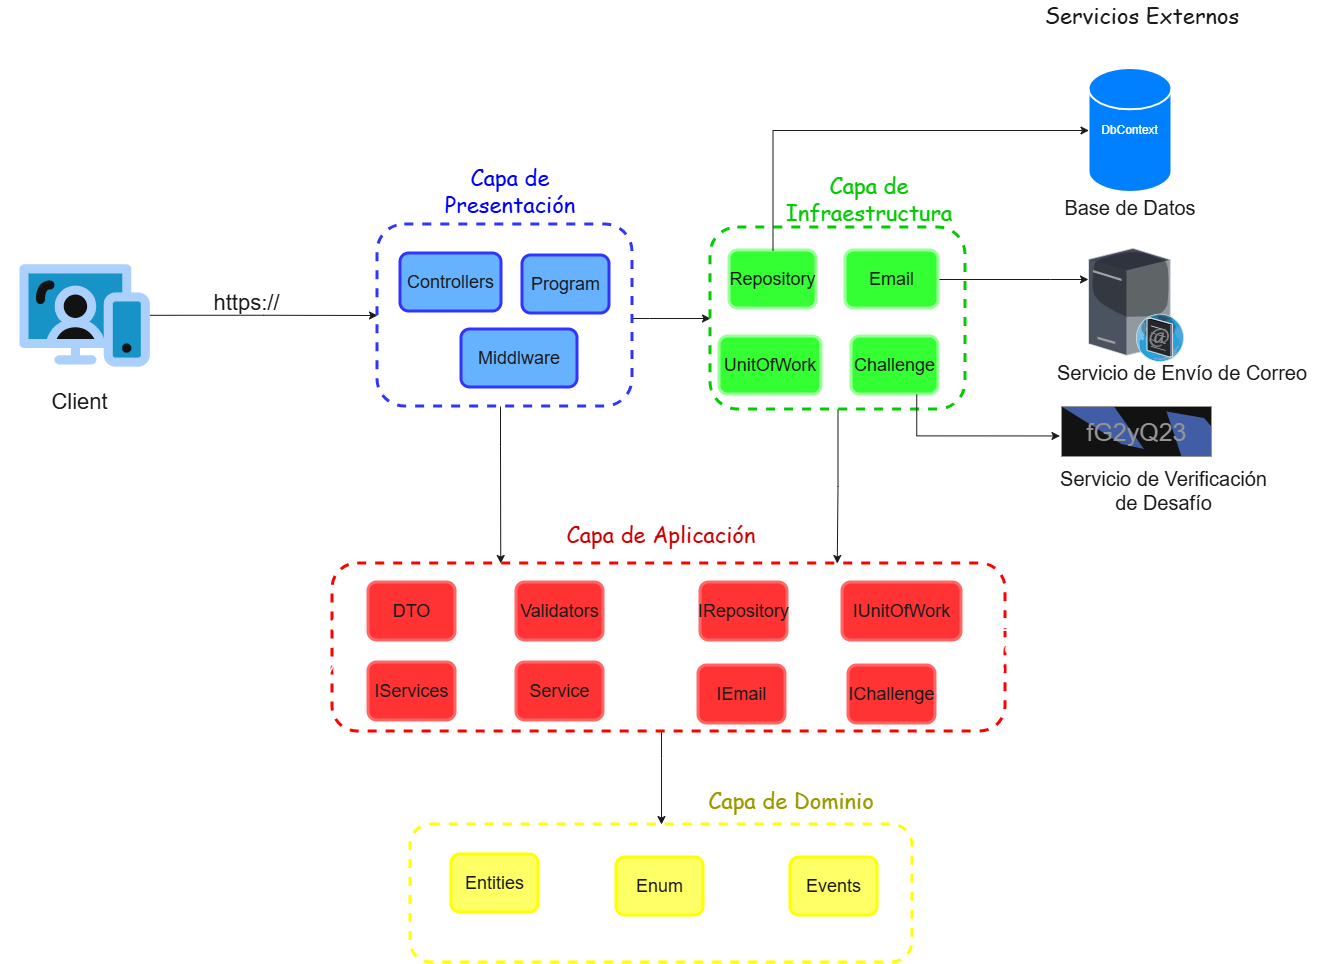
\includegraphics[scale=0.4]{Graphics/Cap3/arquitectura2.drawio.png}
    \caption[Diagrama de la organización del sistema bajo arquitectura limpia]{Diagrama representativo de la organización del sistema bajo un modelo de arquitectura limpia. Fuente: elaboración propia.}
    \label{fig:arquitectura}
\end{figure}

\begin{itemize}
    \item \textbf{Capa de Dominio:} Proyecto central sin dependencias externas. Contiene las entidades de negocio (\texttt{AefiReport}, \texttt{VaccinatedSubject}, \texttt{Vaccine}, \texttt{AdverseEvent}, \texttt{MedicalReviewer}), enumeraciones para clasificación de severidad, estado del paciente.
    
    \item \textbf{Capa de Aplicación:} Depende exclusivamente del proyecto Domain. Contiene los casos de uso organizados según el patrón CQRS: comandos para operaciones de escritura y consultas para lecturas. Define las interfaces de los repositorios, la unidad de trabajo (\texttt{IUnitOfWork}), el servicio de notificaciones (\texttt{INotificationService}), el servicio de envío de correo (\texttt{IEmailSender}), el servicio de verificación de desafío (\texttt{IChallengeVerifier}) y los DTOs para transferencia de datos. Implementa las validaciones de existencia mediante la consulta a repositorios.
    
    \item \textbf{Capa de Infraestructura:} Depende de los proyectos Application y Domain. Proporciona las implementaciones concretas de las interfaces definidas en Application: repositorios con Entity Framework Core sobre MySQL, la unidad de trabajo mediante \texttt{DbContext.SaveChangesAsync}, el servicio de notificaciones, el servicio de envío de correo y el servicio de verificación de CAPTCHA. Contiene además la configuración de autenticación y autorización mediante JWT.
    
    \item \textbf{Capa de Presentación:} Depende del proyecto Application. Corresponde a la API REST desarrollada con ASP.NET Core. Contiene los controladores que reciben las peticiones HTTP, las traducen a comandos o consultas, y retornan las respuestas adecuadas. Implementa las validaciones de formato mediante Data Annotations en los DTOs de entrada. Incluye también la configuración de CORS, Swagger y el middlewares global de excepciones.

\end{itemize}


\subsection{Patrones de Diseño}

La implementación de la Arquitectura Limpia se complementa con un conjunto de patrones de diseño que refuerzan la separación de responsabilidades y la mantenibilidad del sistema. A continuación se describen los más relevantes y se ilustran con fragmentos de código del proyecto.


\subsubsection{Repository}

El patrón Repository abstrae el acceso a los datos mediante una interfaz que simula una colección en memoria, permitiendo al dominio obtener y almacenar objetos sin conocer los detalles de persistencia \cite{evans2003, fowler2002}.

En el proyecto, cada entidad del dominio cuenta con una interfaz de repositorio definida en la capa de Aplicación. La implementación concreta reside en Infraestructura y utiliza Entity Framework Core sobre MySQL. Así, los casos de uso invocan métodos como \texttt{GetByIdAsync} o \texttt{AddAsync} sin depender del \texttt{DbContext} ni del motor de base de datos.

\subsubsection{Unit of Work}

El patrón Unit of Work mantiene el registro de los cambios realizados sobre un conjunto de objetos durante una transacción de negocio y los persiste de forma atómica \cite{fowler2002}.

En el proyecto se implementa mediante la interfaz \texttt{IUnitOfWork} definida en Aplicación. Su implementación en Infraestructura aprovecha el método \texttt{SaveChangesAsync} del \texttt{DbContext} de Entity Framework Core, que por diseño ya actúa como una unidad de trabajo, garantizando que todas las operaciones pendientes se confirmen o se descarten como un solo bloque.

\subsubsection{Inyección de dependencias}

La inyección de dependencias es un patrón mediante el cual un objeto recibe las dependencias que necesita en lugar de instanciarlas directamente, invirtiendo el control de su creación \cite{fowler2004}.

En el proyecto se utiliza el contenedor nativo de ASP.NET Core. En la capa de Presentación se registran todas las interfaces definidas en Aplicación con sus implementaciones concretas en Infraestructura. De este modo, cuando un caso de uso solicita un \texttt{IAefiReportRepository}, el contenedor resuelve automáticamente la implementación concreta, manteniendo las capas internas desacopladas de las externas.

\subsubsection{Mapper}

El patrón Mapper transfiere datos entre dos objetos independientes sin que ninguno conozca la estructura del otro \cite{fowler2002}.

En el proyecto se emplea para convertir entidades de dominio en DTOs y viceversa. Esto evita exponer las entidades fuera de la capa de Aplicación y mantiene el dominio aislado de los formatos de transporte utilizados por la API REST.

\section{Diseño de base de datos}

\subsection{Modelo Entidad-Relación Extendido (MERX)}
% Aquí presentas el diagrama MERX completo con entidades, atributos, 
% claves primarias/foráneas, cardinalidad y herencia (si aplica).

\subsection{Diccionario de datos}
% Descripción detallada de cada tabla: nombre, atributos, tipo de dato, 
% restricciones, valores por defecto, descripción.

\subsection{Normalización}
% Justificas que el esquema cumple con la 3FN (o la que hayas aplicado), 
% mostrando dependencias funcionales y cómo resolviste posibles anomalías.



% \section{Diseño de la interfaz de usuario (UI/UX)}

% \subsection{Pantallas principales}


% \subsection{Justificación de diseño centrado en el usuario}


% \section{Consideraciones de seguridad y privacidad}

% \subsection{Protección de datos sensibles}

% \subsection{Autenticación y autorización}

% \subsection{Protección contra ataques}

% \subsection{Control anti-bot}

% \section{Alternativas de notificación}



